\documentclass[a4paper,10pt]{article}%
%\documentclass[a4paper,10pt]{scrartcl}

\usepackage{float}
\usepackage{graphicx}
\usepackage[utf8]{inputenc}
\usepackage[english]{babel}
\usepackage[left=2cm,right=3cm,bottom=3.5cm,top=3.5cm]{geometry}
\usepackage{natbib}
\usepackage[utf8]{inputenc}


%opening
\title{}
\author{Leonel Exequiel Gómez}


\usepackage{graphicx}
\graphicspath{ {img/} }

%Path in Unix-like (Linux, OsX) format
\graphicspath{ {img/} }



\begin{document}

\maketitle



\section{Introducción}
Implementaremos un experimento basado en el paper de \citet{Alexander2014} y \citet{Ning2016}. 
El objetivo del experimento es dado un conjunto de imágenes de difusión de 
alta calidad, usar la información presente en las mismas para mejorar la 
resolución de imágenes de difusión de menor calidad. Esto es conocido como 
transferencia de calidad de imágenes (o \textit{image quality transfer} del 
término en ingles). 

Usaremos el conjunto de datos de seis sujetos de la base de datos \textit{Human Connectome Project} como nuestra imagen 
de alta calidad. Los mismos tiene una resolución espacial de $x\times x\times x\ mm^3$ con 288 direcciones 
gradientes y 17 b-valores diferentes. En nuestro caso usaremos solo los gradientes con $b=2000\ s/mm^2$. 
Artificialmente generaremos (utilizando el m\'etodo \textit{reslice} de Dipy que hace una interpolación cubica) una 
imagen de difusión de baja calidad por cada uno de los sujetos. Luego mejoraremos la resolución de las misma y la 
compararemos con la original (figura \ref{hr_vs_lr_input}).


\begin{figure}[h]
%\centering
%\includegraphics[width=0.5\textwidth]{hr_vs_lr_input.pdf}
\caption{Corte coronal del sujeto 180937 conjunto de datos $S_0$. A la izquierda la imagen 
original de $12\times12\times12$ y a la derecha su equivalente disminuida en 
resolución de $6\times6\times6$.} 
\label{hr_vs_lr_input}
\end{figure}%


%Utilizaremos un subvolumen de $12\times12\times12$ con 6 valores de gradientes 
%diferentes, todos ellos con $b=2000$.

\section{Experimento}

Dada una imagen en baja resolución predeciremos su equivalente en alta 
resolución. Para ello denotaremos como $Y^{LR}$ a la imagen en baja resolución 
representada como un vector columna de dimensión $N^{vlrb}$ con $N^{vlrb}$ la 
cantidad de voxeles por la cantidad de gradientes de la imagen. Denotaremos 
como $Y^{HR}$ a la imagen en alta resolución representada como un vector 
columna de dimensión $N^{vhrb}$ con $N^{vhrb}$ la cantidad de voxeles por la 
cantidad de gradientes de la imagen. Al igual que \citep{Ning2016} consideramos 
a las imágenes en baja resolución como la versión sub muestreada de su 
equivalente en alta resolución. Luego el modelo de adquisición de la imagen de 
alta resolución lo podemos expresar como

$$  Y^{LR} = GY^{HR} $$

Donde $G$ es la matriz de sub muestreo de la resolución espacial. En 
nuestra implementación obtendremos $G$ entrenando un algoritmo de aprendizaje automático ( \textit{machine learning} en 
ingles) con pares de volúmenes en baja resolución con su correspondiente en alta resolución. Para eso construiremos el 
conjunto de entrenamiento $T=\{x_i, y_i\}_{i}^{|T|}$, donde cada $x_i$ tiene dimensión $N^{vlrb}$ y los $y_i$ 
dimensión $N^{vhrb}$. Utilizaremos la técnica de validación cruzada dejando uno afuera para evaluar los resultados de 
nuestro análisis y tratar de garantizar que sean independientes al conjunto de entrenamiento utilizado. Para 
entrenar usaremos el algoritmo \textit{LinearRegression} de \textit{machine learning}, provisto por la librería 
\textit{Scikit Learn}.


Con el algoritmo \textit{machine learning} computaremos la transformación lineal $G=YX^{\dagger}$ donde $Y$ tiene como 
columnas los $y_i$, $X$ tiene como columnas los $x_i$ y $X^{\dagger}$ es la pseudo inversa de $X$.
%con el conjunto de imágenes que contamos para entrenar
Luego de obtener $G$, planteamos el siguiente problema de optimización convexa para obtener la imagen en alta calidad 
buscada

$$  \min_{Y^{HR}} \{ || G Y^{HR} - Y^{LR} ||^2  \}$$

Dicha optimización la calculamos usando la librería \textit{CVXPY}.
Adicionalmente, forzaremos al algoritmo de optimización a que la señal reconstruida tenga suavidad espacial agregándole 
la semi norma total variación (TV).

$$ ||Y^{HR}||_{TV} = \sum_{x_{ij} \in Y^{HR}} \left\| \left[  \begin{array}{ccc}
x_{i+1,j}  & -x_{i,j} \\
x_{i,j+1}  & -x_{i,j} \end{array} \right]  \right\|$$

En la sección de resultados compararemos la imagen original con la reconstruida por el 
experimento. Luego compararemos los resultados según la iteración de la validación cruzada sobre el conjunto de 
entrenamiento con el que estimamos $G$. De esta manera veremos como se comporta nuestro m\'etodo cuando el conjunto de 
datos con el que contamos para hacer la transferencia de calidad no es tan bueno.

\section{Resultados}

Comparamos la imagen original con la reconstruida usando las siguientes 
métricas:

\begin{itemize}
% \item Error cuadrático medio por parámetro DTI: Tomamos la imagen en su 
%representación DTI y calculamos el error cuadrático medio de todos los voxeles 
%del volumen por cada uno de los seis parámetros del modelo DTI.
 \item Error cuadrático medio por voxel: Tomamos la imagen en su 
representación DWI y calculamos el error cuadrático medio ($ECM$) por cada voxel del 
volumen.
%$$\frac{1}{160} \sum_{i=1}^{160} (S_{reconstruida}(q_i)-S_{original}(q_i))^2 $$ 
 \item Error cuadrático medio por gradiente: Tomamos la imagen en su 
representación DWI y calculamos el error cuadrático medio de todos los voxeles 
por cada gradiente. Esta métrica nos permite observar cuanto dista la imagen 
reconstruida con la original según el gradiente.
 \item Coeficiente de determinación: El Coeficiente de Determinación, es el cuadrado del 
coeficiente de correlación de Pearson. Nos da la proporción de variación de la variable a predecir. 
Si la proporción es igual a 0, quiere decir que el modelo no es bueno. Si esta cerca de uno 
quiere decir que el modelo es bueno y para valores negativos significa que nuestro conjunto de 
datos no se comporta de manera lineal.
 %\item Histograma: Calculamos el histograma de una rebanada coronal para un 
%b-valor nulo y uno no nulo. Ver el histograma de una imagen nos ayuda analizar 
%sobre el contrastarte de la misma.
\end{itemize}


En la figura \ref{resultado} se ve el resultado del algoritmo de optimización con la regularización de la norma TV.

\begin{figure}[H]
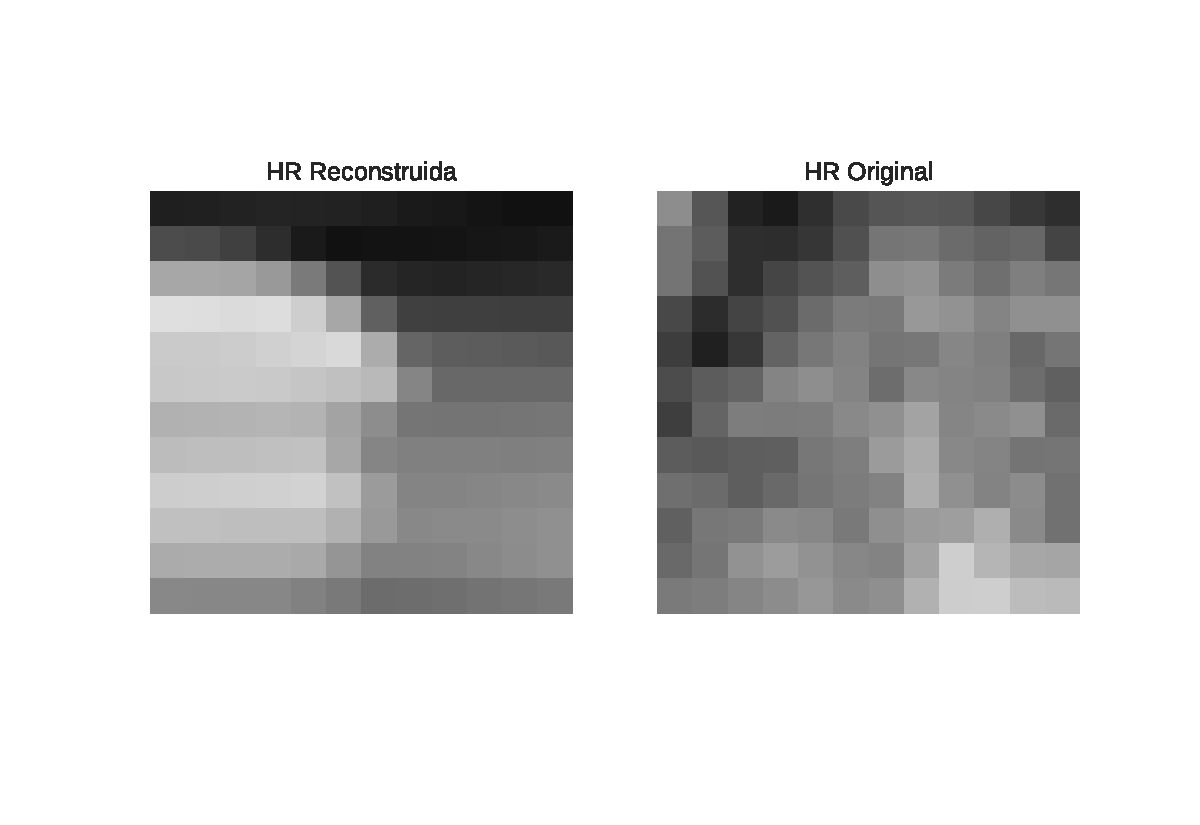
\includegraphics[scale=0.8]{Yhr_compare_s180129.pdf}
\caption{Resultado de la reconstrucción usando la norma TV. }
\label{resultado}
\end{figure}


Además probamos el resultado del algoritmo de \textit{machine learning} reconstruyendo el 
volumen de baja resolución de la siguiente manera

$$\widehat{Y^{LR}} = GY^{HR}$$

En la tabla \ref{tab:res} podemos ver el valor mínimo alcanzado por el algoritmo de minimización, el 
tiempo de ejecución del mismo, y las normas de la imagen estimada y la diferencia entre la estimada 
y la original. 




\begin{table}[H]
\centering
\begin{tabular}{ |c|c|c|c|c|c|c| }
 \hline
 tv & $||\widehat{Y^{HR}}||$ & $||Y^{HR}||$& $||\widehat{Y^{LR}}||$ &$||Y^{LR}||$ & $||\widehat{Y^{HR}}-Y^{HR}||$& 
$||\widehat{Y^{LR}}-Y^{LR}||$\\
 \hline 
 si & $100050\pm17750$ & $13164\pm3057$  & $48974\pm12775$ & $48974\pm12775$ & 
$48974\pm12775$ & $48974\pm12775$ \\
 no & $17926\pm20$ & $6433\pm15$ & $811\pm3$ & $48974\pm12775$ & $48974\pm12775$  & 
$48974\pm12775$\\
 \hline
\end{tabular}

\caption{La norma de la imagen estimada, la original y la norma de la diferencia entre la estima y la original, de la 
imagen con alta resolución y baja resolución.}
\label{tab:res}
\end{table}


\begin{table}[H]
\centering
\begin{tabular}{ |c|c|c| }
 \hline
 tv & Valor Óptimo & tiempo \\
 \hline 
 si &$226618\pm75970$  & $0'24''$  \\
 no &$3058\pm530$  & $5'02''$  \\
 \hline
\end{tabular}

\caption{El valor alcanzado por el algoritmo de minimización y  el tiempo de ejecución.}
\label{tab:res_time}
\end{table}

La figura \ref{mse_cmp} muestra una rebanada coronal de la imagen de difusión original, la producida 
por el m\'etodo y el error cuadrático medio entre las \'ultimas dos. Como 
podemos apreciar solo algunos voxeles toman valores relativamente altos en la 
imagen $ECM$.

\begin{figure}[H]
\centering        
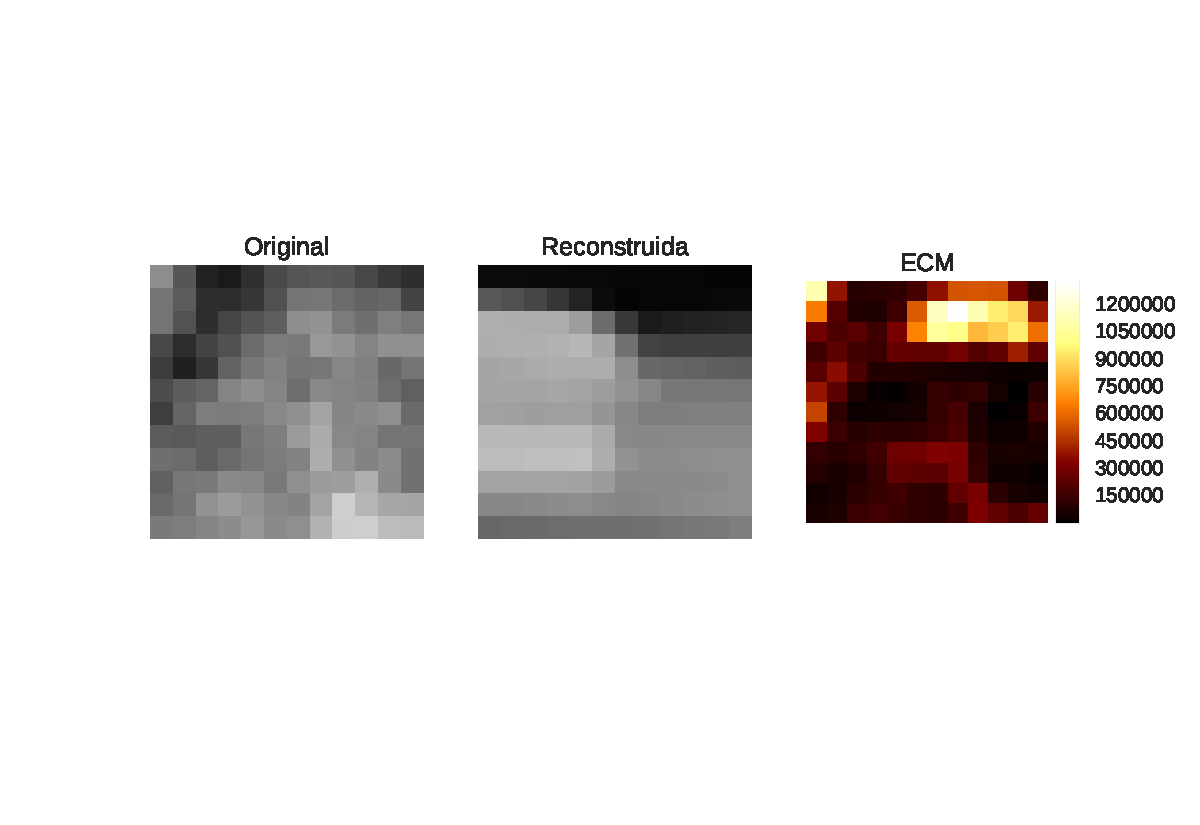
\includegraphics[scale=0.7]{mse_yhr_s180937_voxels_cmp.pdf}
\caption{De izquierda a derecha una rebanada coronal de la imagen 
original, la producida por el m\'etodo y el error cuadrático medio por voxel de la 
representación DWI de la imagen. La imagen fue resultado de la iteración que dejo afuera al sujeto 180937.}
\label{mse_cmp}
\end{figure}


La figura \ref{cdet_cmp} muestra también una rebanada coronal de la imagen 
original, la producida por el m\'etodo y el coeficiente de determinación entre las \'ultimas dos. 
Dicho coeficiente nos aporta información de cuan bueno fue el modelo que utilizamos para ajustar 
los datos. En nuestro caso el modelo usado fue lineal y gran parte de los voxeles presentan un 
coeficiente de determinación negativo. Esto significa que el modelo elegido no se comporta de manera lineal.

\begin{figure}[H]
\centering        
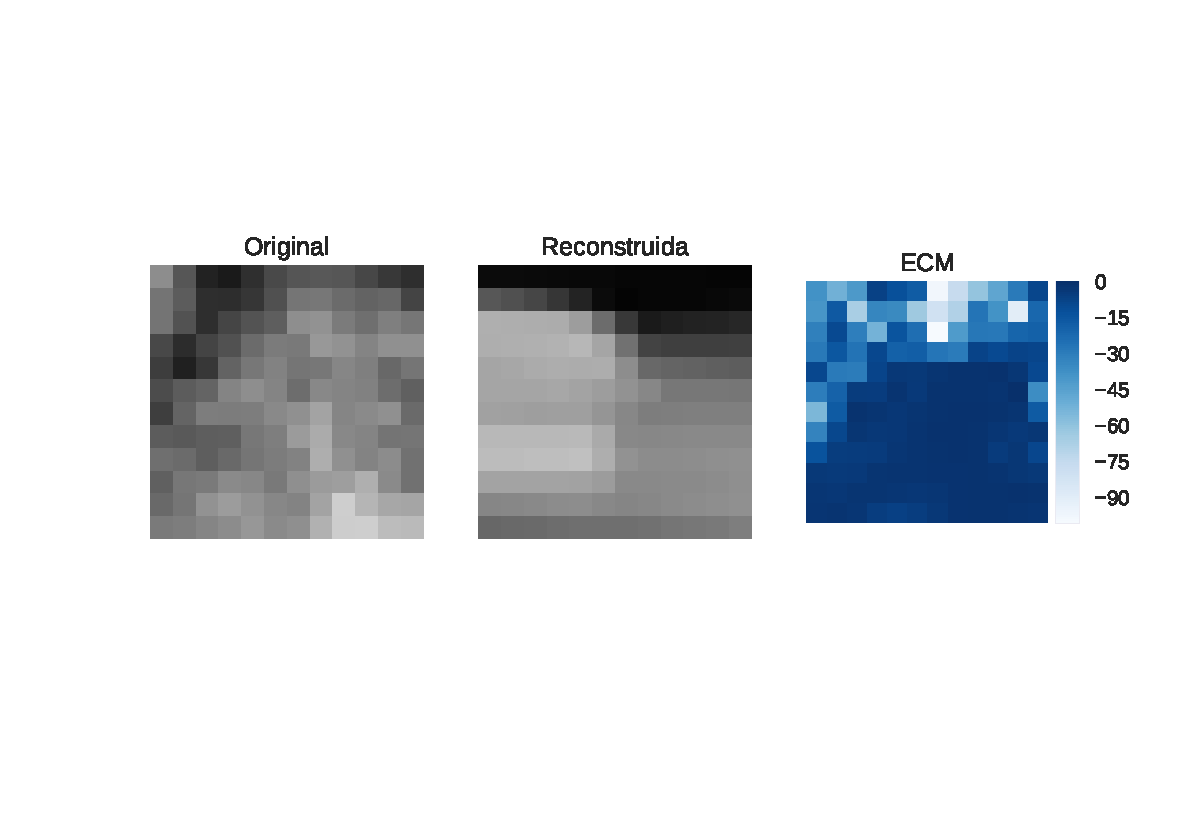
\includegraphics[scale=0.7]{cdet_yhr_s180937_voxels_cmp.pdf}
\caption{De izquierda a derecha una rebanada coronal de un gradiente arbitrario de la imagen 
original, la producida por el m\'etodo y el coeficiente de determinación por voxel de la 
representación DWI de la imagen. La imagen fue resultado de la iteración que dejo afuera al sujeto 180937.}
\label{cdet_cmp}
\end{figure}


En la figura \ref{error_norma} graficamos la norma del error cometido en la reconstrucción tanto del volumen con 
alta resolución y con baja resolución.


\begin{figure}[H]
%\centering        
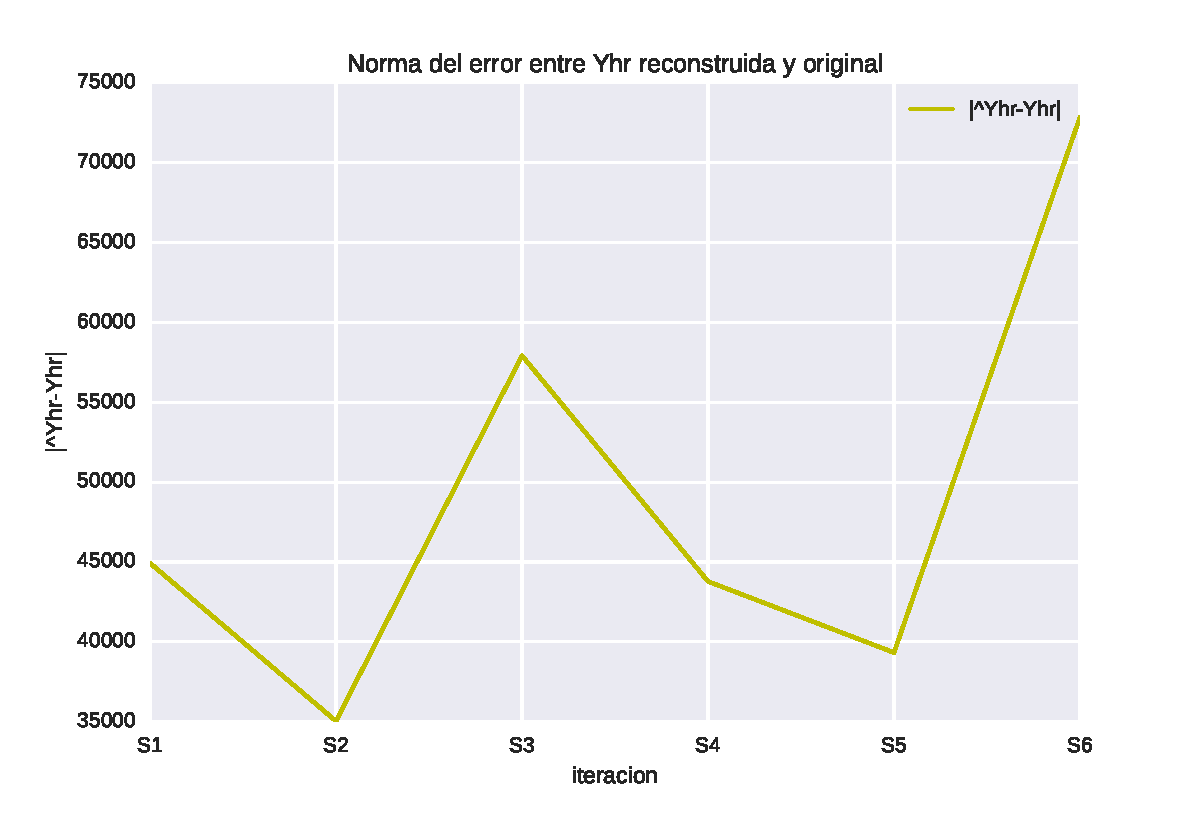
\includegraphics[scale=0.4]{norma_error_yhr.pdf}
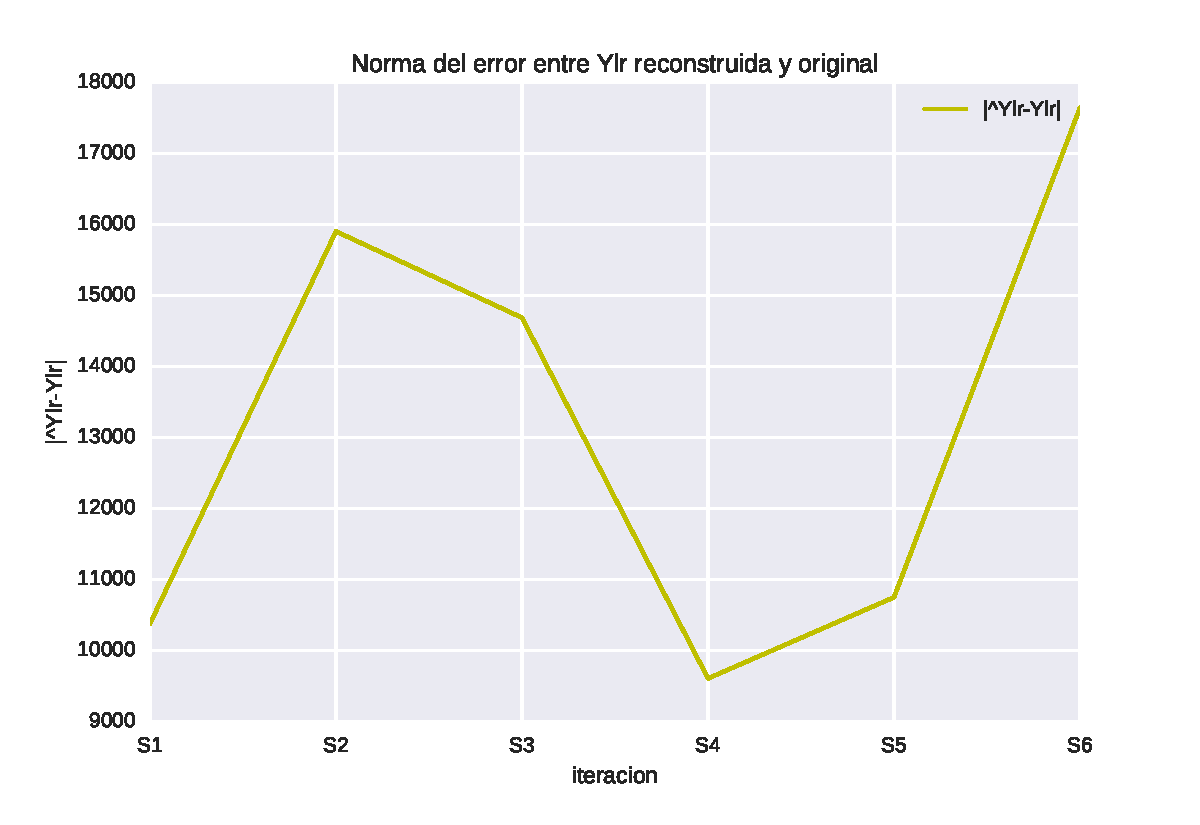
\includegraphics[scale=0.4]{norma_error_lr.pdf}

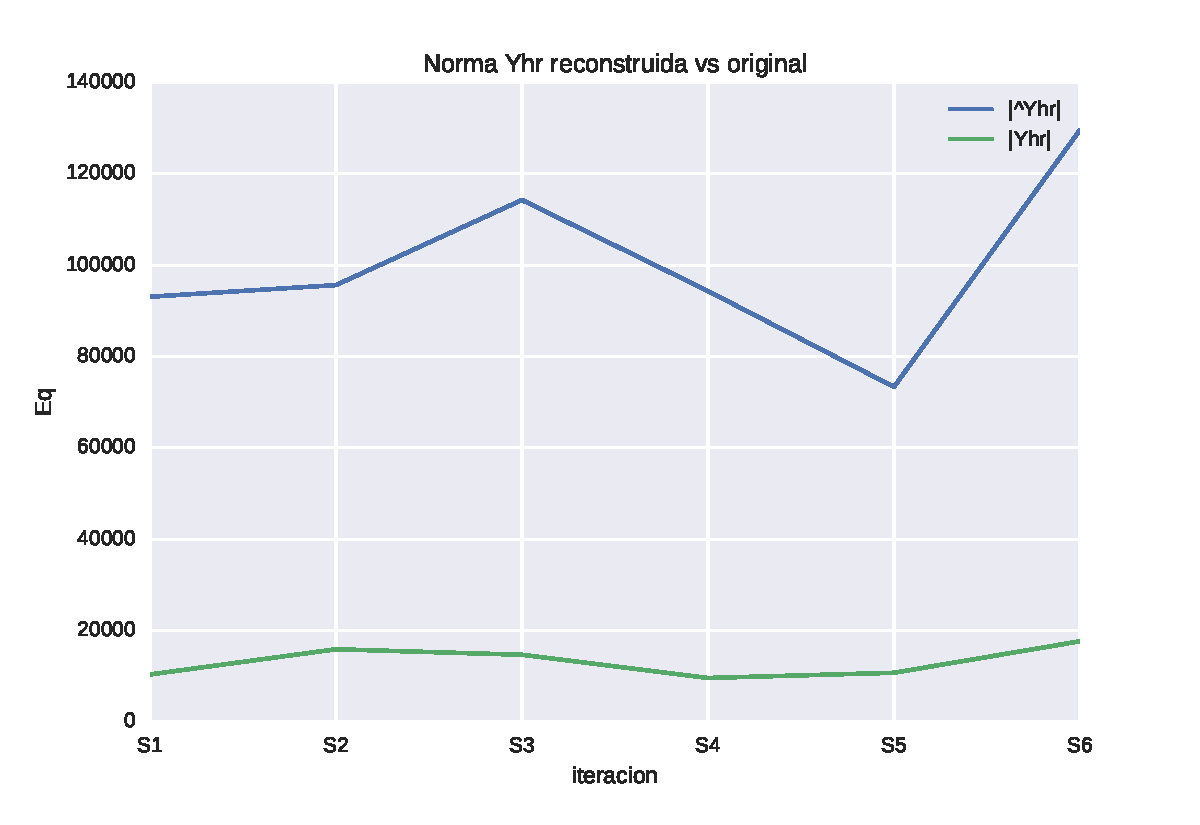
\includegraphics[scale=0.4]{cmp_normas_yhr.pdf}
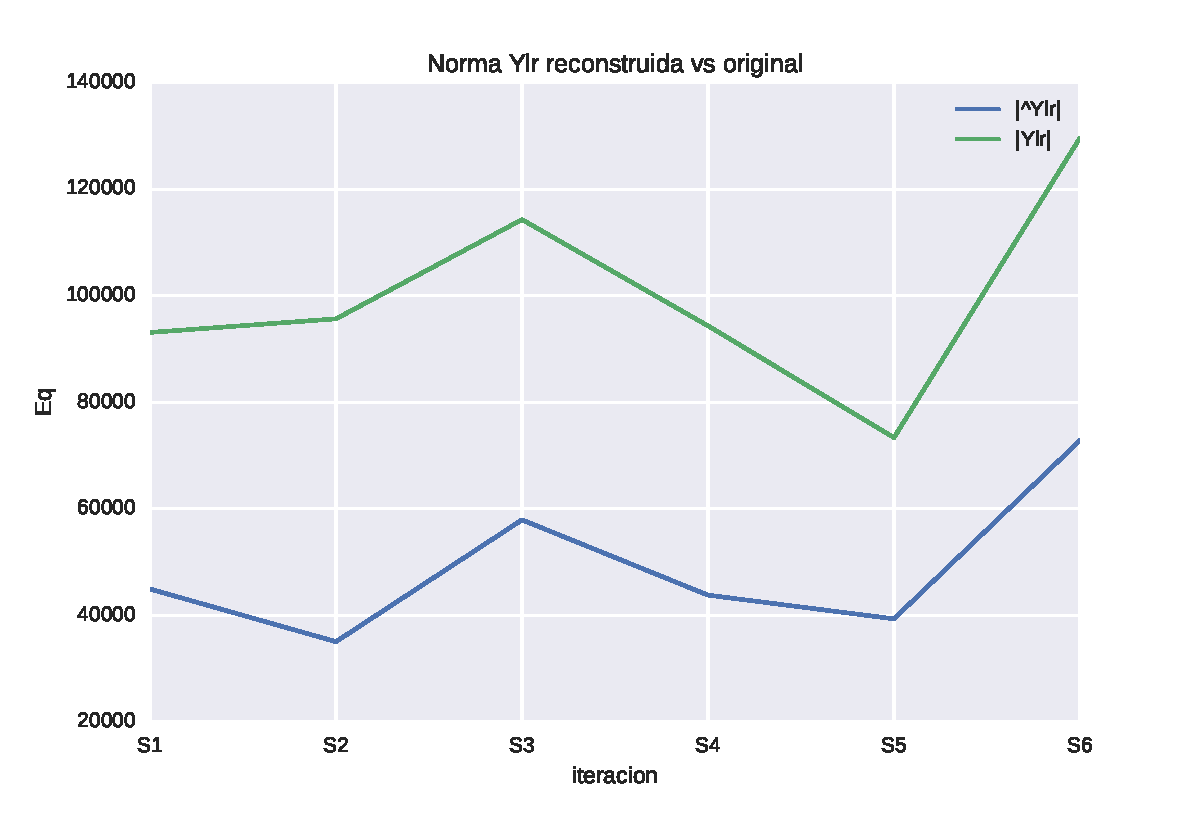
\includegraphics[scale=0.4]{cmp_normas_ylr.pdf}
\caption{Arriba la norma de la diferencia entre los volúmenes reconstruidos y los originales. Abajo la comparación 
entre el valor de sus normas por cada iteración realizada. }
\label{error_norma}
\end{figure}


Finalmente en la figura \ref{opt_vals} vemos el mínimo valor encontrado por el algoritmo para nuestra expresión.

\begin{figure}[H]
\centering        
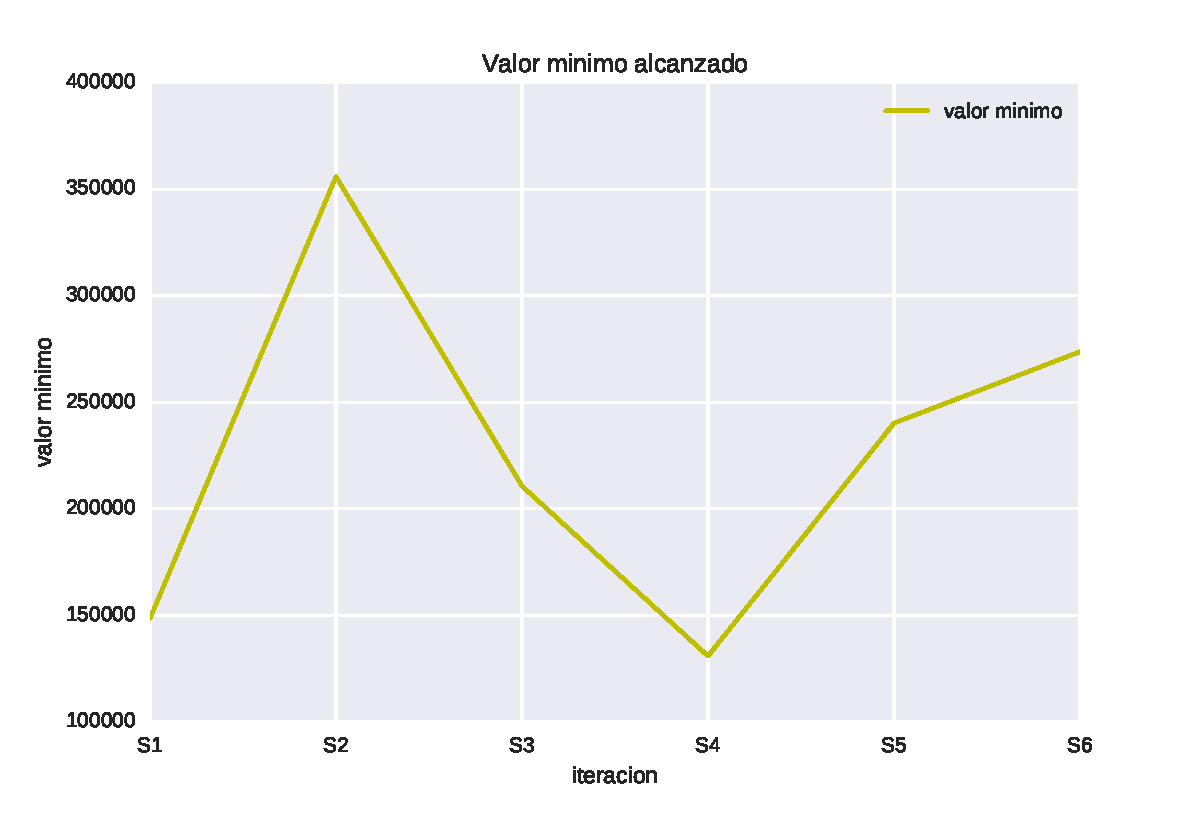
\includegraphics[scale=0.7]{opt_vals.pdf}
\caption{El valor mínimo alcanzado por el algoritmo de optimización en cada iteración realizada. }
\label{opt_vals}
\end{figure}


\begin{figure}[H]
%\centering        
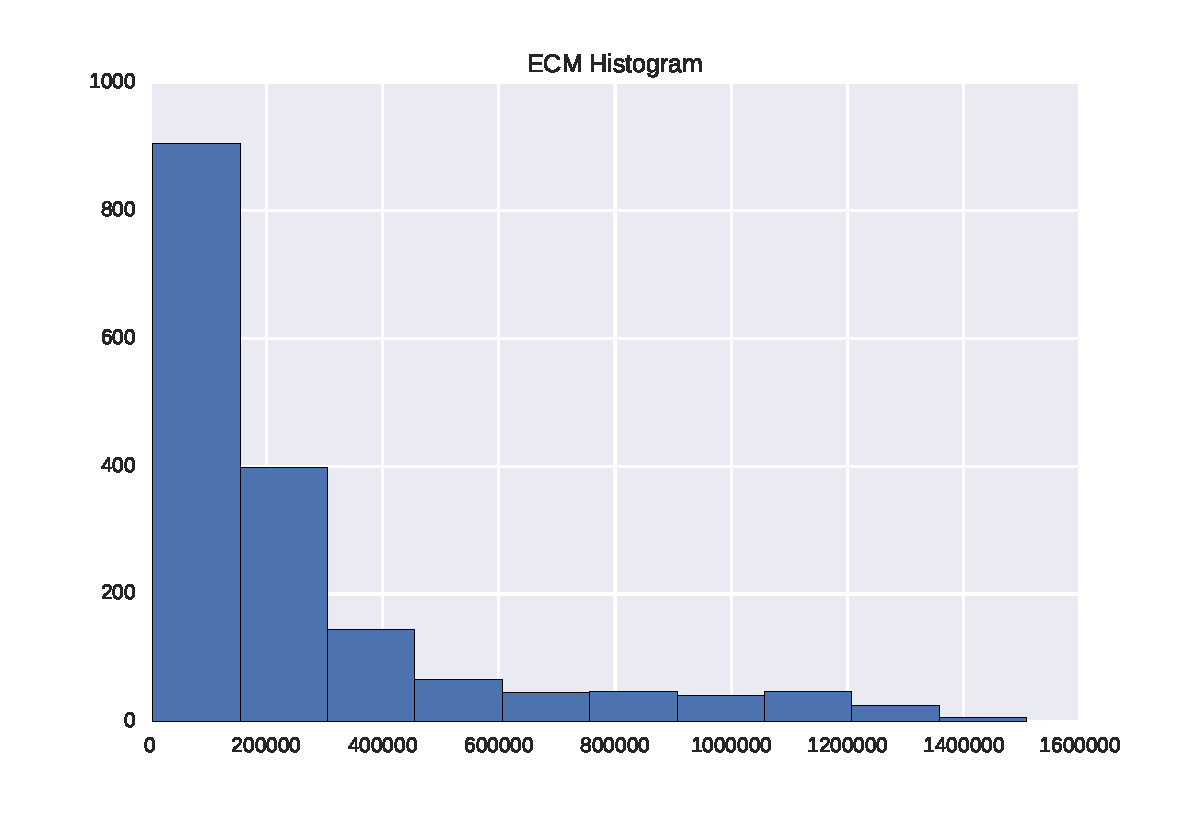
\includegraphics[scale=0.4]{mse_hist_s180937.pdf}
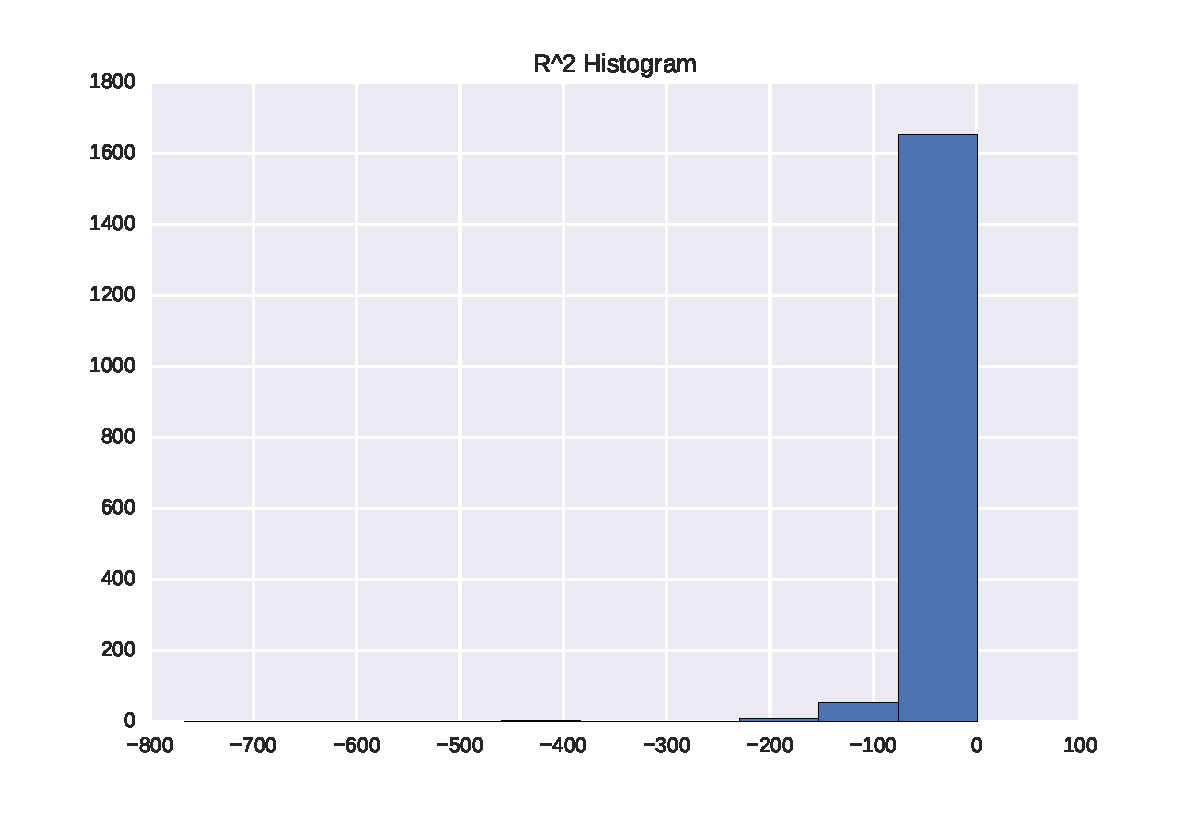
\includegraphics[scale=0.4]{cdet_hist_s180937.pdf}
%\caption{El valor minimo alcanzado por el algoritmo de optimización en cada iteración realizada. }
%\label{opt_vals}
\end{figure}


\begin{figure}[H]
\centering        
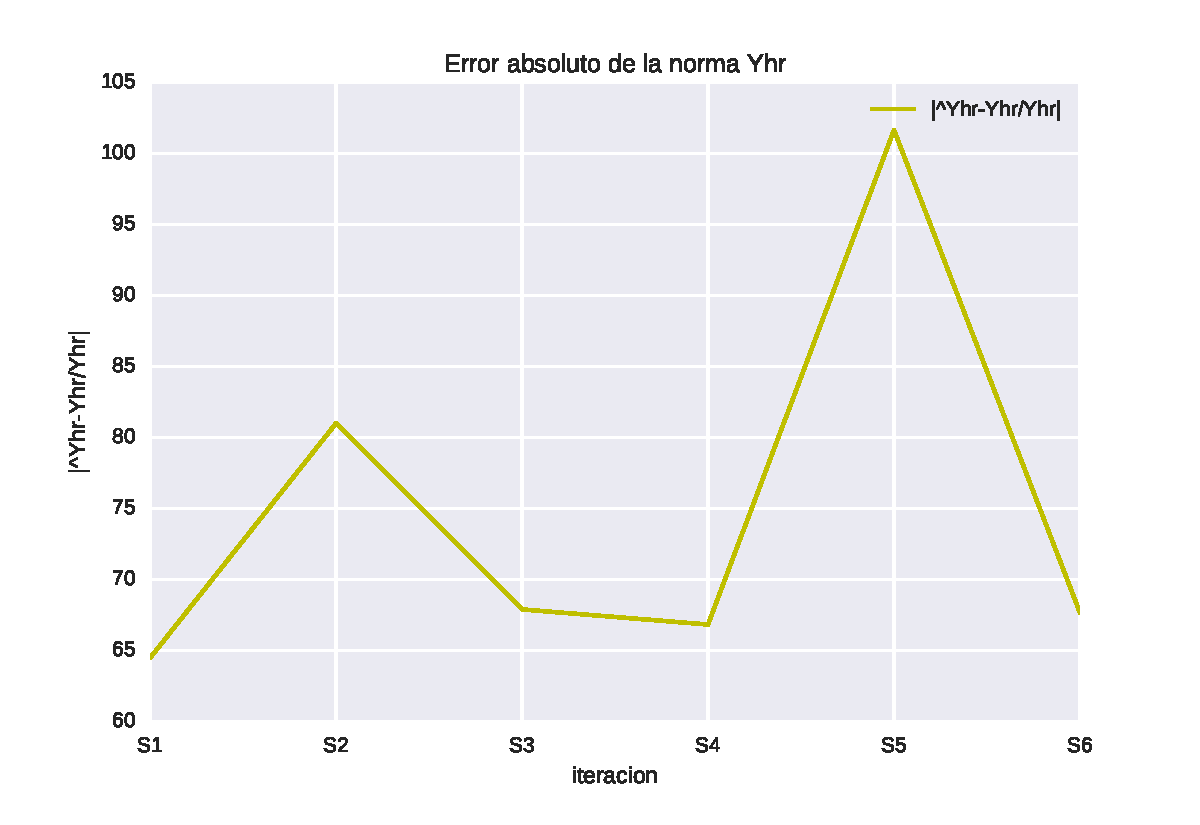
\includegraphics[scale=0.7]{eabs_norma_yhr.pdf}
\caption{Error relativo de la imagen en alta resolución reconstruida. }
%\label{opt_vals}
\end{figure}


\clearpage
\section{Conclusiones}
%
En el caso de los b-valores altos el error es m\'as abrupto en las regiones donde predomina el 
tejido isotrópico (como la materia gris, csf, etc).




El modelo propuesto se comporta bien para valores no tan altos de relación señal ruido. Como se ve 
en la figura \ref{mse_por_gradientes_by_snr_todos} cuando la relación señal ruido es 
inferior a 50 el error del método crece abruptamente. 

A simple vista (incluso los resultados con $SNR=25$) el modelo aproxima bien la 
imagen en cuanto a graficar la señal de difusión. Es decir, que respeta 
bastante bien el contraste entre voxeles. Más allá de que las magnitudes de los 
mismos difieran con las de la original y eso cause diferencias sensibles al 
calcular el $ECM$. Habría que probar estos resultados al intentar 
usar los datos para hacer cosas mas complejas como por ejemplo un tractograma.

%\clearpage
%\section{Apendice}
%

Sean:

 $ vhr \in  Z_{ \geq 0} $
 
 $ bval \in  Z_{ \geq 0} $
 
 $Y^{hr} \in \Re^{vhr\times bval}$
 
 $Y^{lr} \in \Re^{vlr\times bval}$

 $G \in \Re^{vlr\times vhr}$


$$  \min_{Y^{hr}} \{ || G Y^{hr} - Y^{lr} ||^2  \}$$

Llamo a :

$f : \Re^{vhr\times bval} \rightarrow \Re^{vlr\times bval}$

$$f(Y^{hr}) = G Y^{hr} - Y^{lr} $$

$g:\Re^{vhr\times bval} \rightarrow \Re$

$$g(Y^{hr}) = ||f(Y^{hr})||^2 $$

con 

$f_{ij}(Y^{hr}) : \Re$

$$f_{ij}(Y^{hr}) = (\sum_{k=1}^{vhr} G_{ik} Y_{kj}^{hr}) - Y_{ij}^{lr} $$

Luego

$$g(Y^{hr}) = [ \sqrt{ \sum_{i=1}^{vlr} \sum_{j=1}^{bval} f_{ij}^2 (Y^{hr})} ]^2 $$


$$g(Y^{hr}) =  \sum_{i=1}^{vlr} \sum_{j=1}^{bval} f_{ij}^2 (Y^{hr}) $$


Para minimizar $g(Y^{hr})$ preciso $\nabla g \in \Re^{vhr\times bval} $.
Si nos enfocamos en un componente del gradiente, osea la derivada parcial con respecto a 
$Y_{ij}^{hr}$, al ser una sumatoria solo afecta a la derivada los sumandos que tiene a 
$Y_{ij}^{hr}$ es decir:

$$\frac{\partial g (Y^{hr})}{\partial Y_{ij}^{hr}} = \sum_{k=1}^{vlr} \frac{\partial 
f_{kj}^2(Y^{hr})}{\partial Y_{ij}^{hr}}$$



Por la derivada de la composición $(g \circ h)' (Y^{hr}) = g'(h(Y^{hr})) \ 
h'(Y^{hr})$ tenemos que 

$$\frac{\partial g (Y^{hr})}{\partial Y_{ij}^{hr}} = \sum_{k=1}^{vlr} 2 f_{kj}(Y^{hr}) 
\frac{\partial 
f_{kj}(Y^{hr})}{\partial Y_{ij}^{hr}}$$

y 


$$\frac{\partial f_{kj}(Y^{hr})}{\partial Y_{ij}^{hr}} = 0 + 0 + \cdots + 
\underbrace{(G_{ki}Y_{ij}^{hr})'}_{k=i} + 0 + \cdots $$

$$\frac{\partial f_{kj}(Y^{hr})}{\partial Y_{ij}^{hr}} = G_{ki}$$

luego



$$\frac{\partial g (Y^{hr})}{\partial Y_{ij}^{hr}} = \sum_{k=1}^{vlr} 2 f_{kj}(Y^{hr})G_{ki}$$


$$\frac{\partial g (Y^{hr})}{\partial Y_{ij}^{hr}} = \sum_{k=1}^{vlr} 2 [(\sum_{p=1}^{vhr} G_{kp} 
Y_{pj}^{hr}) - Y_{kj}^{lr}] G_{ki}$$



$$\frac{\partial g (Y^{hr})}{\partial Y_{ij}^{hr}} = 2 \sum_{k=1}^{vlr} G_{ki} (\sum_{p=1}^{vhr} 
G_{kp} 
Y_{pj}^{hr}) - Y_{kj}^{lr}$$



que equivale a su forma matricial


$$\nabla g (Y^{hr}) = 2 G^t(G Y^{hr}-Y^{lr})$$





\clearpage
\bibliographystyle{plainnat}
\bibliography{references.bib}



\end{document}
